\chapter{Grafana}

Grafana is an open-source platform for monitoring and observability. It allows you to query, visualize, alert on, and understand your metrics no matter where they are stored. In this project, Grafana is used to visualize the database data and analytics.

\begin{figure} [H]
    \centering
    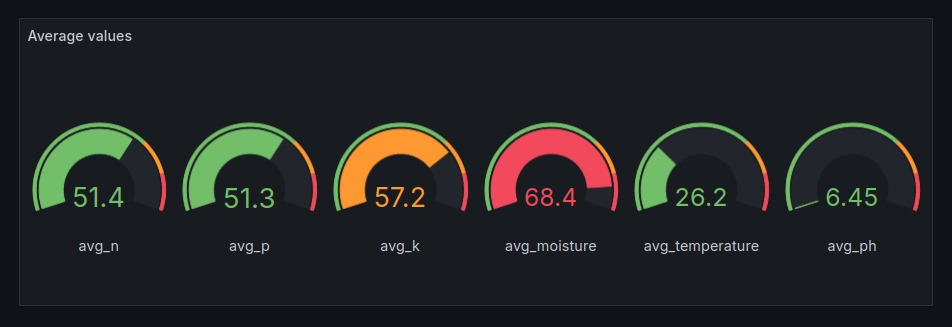
\includegraphics[width=0.8\textwidth]{media/grafana_4.jpg}
    \caption{Graphic showing the average of plant growth parameters such as temperature, pH, humidity, and nutrients (N, P, K) for each field.}
    \label{fig:grafana}
\end{figure}


\begin{figure} [H]
    \centering
    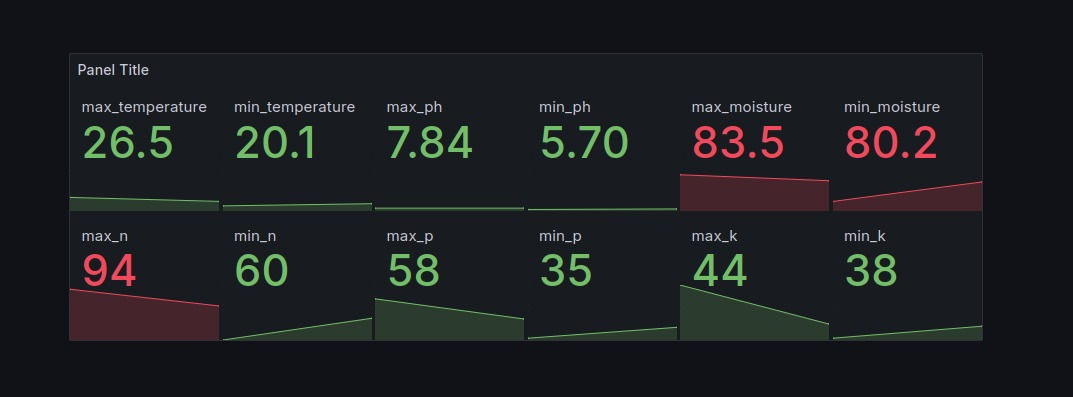
\includegraphics[width=0.8\textwidth]{media/grafana_3.jpg}
    \caption{Graphic showing maximum and minimum statistics for various plant growth parameters such as temperature, pH, humidity, and nutrients (N, P, K), grouped by sowing state.}
    \label{fig:grafana}
\end{figure}